% Emacs settings: -*-mode: latex; TeX-master: "manual.tex"; -*-

\section{Simple optical components:
Arms, slits, collimators, filters}
Below we list a number of simple optical components 
which require only a minimum of explanation.

\subsection{Arm: The generic component}
\label{explain:arm}
The component {\bf Arm} is empty; is resembles an optical bench
and has no effect on the neutron.
The function of this component is only to set up a local frame of
reference within the instrument definition. Other components of the
same arm/optical bench may then be
positioned relative to the arm component
using the \MCS\ meta-language.
The use of arm components in the instrument definitions
is not required but is recommended for clarity.

{\bf Arm} has no input parameters.
For more about the use of this component, see the 
sample instrument definitions listed in Appendix \ref{instcode}.


\subsection{Slit: The rectangular slit}
\label{slit}
The component {\bf Slit} is a very simple construction.
It sets up a rectangular opening at $z=0$, and propagates the neutrons 
onto the plane of this rectangle by the kernel call PROP\_Z0.

Neutrons within the slit opening are unaffected, 
while all other neutrons
(no matter how far from the opening their paths intersect the plane)
are discarded by the kernel call ABSORB.
By this simplification, some neutrons contributing to the background
in a real experiment will be neglected. 
These are the ones that scatter off the inner side
of the slit, penetrates the slit material, 
or that clear one of the outer edges of the slit.

The input parameters of {\bf Slit} are the four coordinates,
$(x_{\rm min}, x_{\rm max}, y_{\rm min}, y_{\rm max})$
defining the opening of the rectangle.

\subsection{Circular\_slit: The circular slit}
The component {\bf Circular\_slit} defines a circle in the $z=0$ plane,
centered in the origin. In analogy with {\bf Slit},
neutrons are propagated to this plane, and those which intersect
the plane outside the circle are ABSORB'ed.

The only input parameter of {\bf Circular\_slit} is
the radius, $r$, of the circle.

\subsection{Beamstop\_rectangular: The rectangular beam stop}
\label{s:Beamstop_rectangular}
The component {\bf Beamstop\_rectangular} models a thin, infinitely
absorbing rectangle in the $X$-$Y$ plane, centered on the origin. The
input parameters are \textit{xmin}, \textit{xmax}, \textit{ymin}, and
\textit{ymax} defining the edges of the slit in meters.


\subsection{Beamstop\_circular: The circular beam stop}
\label{s:Beamstop_circular}
The component {\bf Beamstop\_circular} models a thin, infinitely
absorbing circular disk in the $X$-$Y$ plane, centered on the origin. It
takes a single input parameter \textit{radius} to define the circle
radius in meters.


\subsection{Soller: The simple Soller blade collimator}
The component {\bf Soller} defines two rectangular openings
like the one in {\bf Slit}. Neutrons not clearing both these
openings are ABSORB'ed, see the discussion in \ref{slit}.
The collimating effect is taken care of by employing an ideal
triangular transmission through the collimator, as explained below.
For a more detailed Soller collimator simulation the Channeled\_guide
component can be employed, see section~\ref{s:channeled_guide}.

Let the collimation angle be $\delta = \tan^{-1}(d/L)$,
where $L$ is the length of the collimator
and $d$ is the distance between the blades,
and let $\phi$ be the divergence angle between the 
neutron path and a vertical plane along the collimator axis, 
see Fig.~\ref{f:collimator}. Neutrons with a large 
divergence angle $|\phi| \geq \delta$ will always
hit at least one collimator blade and will thus be absorbed.
For smaller divergence angles, $|\phi| < \delta$, the fate of the
neutron depends on its exact entry point.
Assuming that a typical collimator has many blades, the
absolute position of each blade perpendicular to the collimator axis
is somewhat uncertain (and also unimportant).
A simple statistical consideration now shows that the transmission
probability is $T = 1-\tan|\phi|/\tan\delta$.

\begin{figure}
  \begin{center}
    \psfrag{xmin}[c][c]{$x_{\rm min}$}
    \psfrag{xmax}[c][c]{$x_{\rm max}$}
    \psfrag{ymin}[c][c]{$y_{\rm min}$}
    \psfrag{ymax}[c][c]{$y_{\rm max}$}
    \psfrag{delta}[c][c]{$\delta$}
    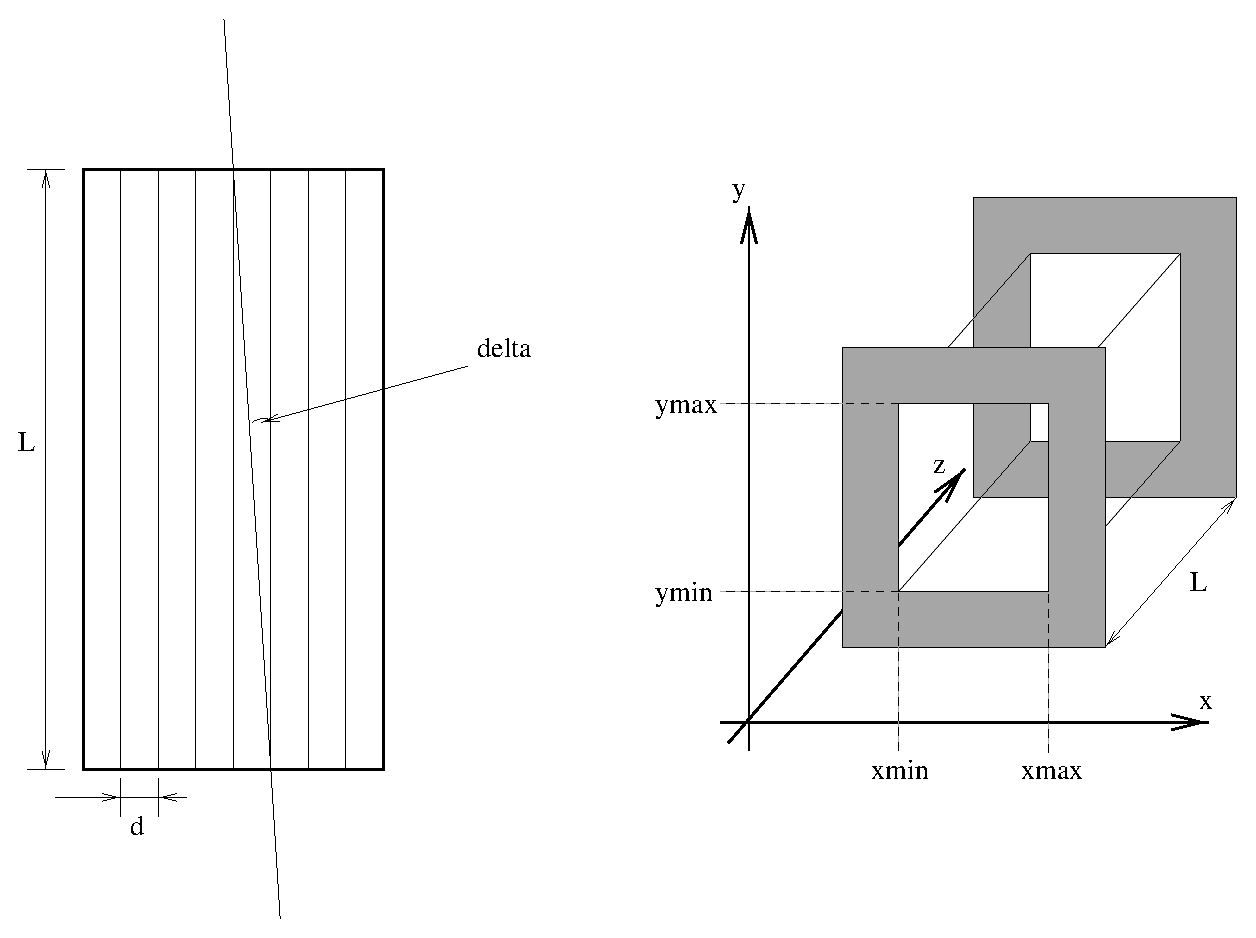
\includegraphics[width=0.9\textwidth]{figures/collimator.eps}
  \end{center}
\caption{The geometry of a simple Soller blade collimators:
The real Soller collimator, seen from the top (left), 
and a sketch of the component {\bf Soller} (right).
The symbols are defined in the text.}
\label{f:collimator}
\end{figure}

We simulate the collimator by transmitting all neutrons with
$|\phi| < \delta$, but adjusting their weight with the amount
\begin{equation}
\pi_i = T = 1-\tan|\phi|/ \tan\delta ,
\end{equation}
while all others are discarded by the kernel call ABSORB.

The input parameters for {\bf Soller} are the coordinates
$(x_{\rm min}, x_{\rm max}, y_{\rm min}, y_{\rm max})$,
defining the identical entry and exit apertures, 
the length, $l$, between the slits, 
and the collimator divergence $\delta$.
If $\delta=0$, the collimating effect is disabled,
so that $\pi_i = 1$ whenever the neutron clears the two apertures.

\subsection{Filter: A transmission filter}
A neutron transmission filter act in much of the same way as two
identical slits, one after the other.
The only difference is that the transmission of the filter
varies with the neutron energy.

In the simple component {\bf Filter},
we have not tried to simulate the details of the transmission
process (which includes absorption, incoherent scattering,
and Bragg scattering in a polycrystalline sample, {\em e.g.} Be).
Instead, the transmission is parametrised to be
$\pi_i=T_0$ when $E \leq E_{\rm min}$, $\pi_i=T_1$ when $E \geq E_{\rm max}$,
and linearly interpolated between the two values
in the intermediate interval.
\begin{equation}
\pi_i = \left\{ \begin{array}{lc}
 T_0  & E \leq E_{\rm min} \\
 T_1 + (T_0-T_1) \frac{E_{\rm max}-E}{E_{\rm max}-E_{\rm min}}
 & E_{\rm min} < E < E_{\rm max} \\
 T_1  & E_\geq E_{\rm max} \\
\end{array} \right.
\end{equation}
If $T_1=0$, the neutrons with $E>E_{\rm max}$ are ABSORB'ed.

The input parameters are the four slit coordinates, 
$(x_{\rm min}, x_{\rm max}, y_{\rm min}, y_{\rm max})$,
the distance, $l$, between the slits, and the transmission parameters 
$T_0$, $T_1$, $E_{\rm min}$, and $E_{\rm max}$. 
The energies are given in meV.
